\documentclass[t,18pt]{beamer}
\usepackage[utf8]{inputenc}

\author{Christian Schnorr}
\title{Minimizing Potential Energy\\ in Constrained Physical Systems\\ and Applications to Graph Drawing}
\date{April 25th, 2017}

\usepackage{algorithm2e}
\SetKwInput{KwData}{Input}
\SetKwInput{KwResult}{Output}
\DontPrintSemicolon

\newcommand{\code}{\texttt}

% Talk is 25 minutes + 5 minutes of questions.

\usetheme{Rochester}

\setbeamercolor{normal text}{fg=black}
\setbeamercolor{frametitle}{fg=white}

\newcommand{\light}[1]{\textcolor{black!40}{#1}}

\makeatletter
\setbeamertemplate{footline}
{
  \leavevmode%
  \hbox{%
  \begin{beamercolorbox}[wd=.5\paperwidth,ht=2.25ex,dp=1ex,center]{author in head/foot}%
    \usebeamerfont{author in head/foot}\insertshortauthor
  \end{beamercolorbox}%
  \begin{beamercolorbox}[wd=.5\paperwidth,ht=2.25ex,dp=1ex,right]{date in head/foot}%
    \usebeamerfont{date in head/foot}\insertshortdate{}\hspace*{2em}
    \insertframenumber{} / \inserttotalframenumber\hspace*{2ex}
  \end{beamercolorbox}}%
  \vskip0pt%
}
\makeatother

\usepackage{amsmath}
\usepackage{amssymb}
\usepackage{mathtools}


% Functions

\newcommand{\eval}[2]{{#1}{\left({#2}\right)}}
\newcommand{\floor}[1]{\left\lfloor#1\right\rfloor}
\newcommand{\ceil}[1]{\left\lceil#1\right\rceil}


% Algebra

\newcommand{\abs}[1]{\left\lvert#1\right\rvert}
\newcommand{\norm}[1]{\left\lVert#1\right\rVert}


% Calculus

\newcommand{\differential}[1]{\mathop{d #1}}


% Geometry

\newcommand{\segment}[1]{\overline{#1}}
\newcommand{\longvec}[1]{\overrightarrow{#1}}
\newcommand{\degrees}{^{\circ}}


% Big O notation

\newcommand{\bigOh}[1]{\mathcal{O}(#1)}
\newcommand{\bigTheta}[1]{\Theta(#1)}
\newcommand{\bigOmega}[1]{\Omega(#1)}


% Graph Theory

\newcommand{\indeg}{deg^{-}}
\newcommand{\outdeg}{deg^{+}}


% Set Theory

\newcommand{\cupplus}{\uplus}

% \usepackage{amsthm}
\usepackage{float}
\usepackage[inline]{enumitem}

\theoremstyle{definition}
\newtheorem{definition}{Definition}

\theoremstyle{definition}
\newtheorem{theorem}{Theorem}

\theoremstyle{definition}
\newtheorem{lemma}{Lemma}

\theoremstyle{definition}
\newtheorem{proposition}{Proposition}

\theoremstyle{definition}
\newtheorem{corollary}{Corollary}

\theoremstyle{definition}
\let\oldproofname=\proofname
\renewcommand{\proofname}{\rm\bf{\oldproofname}}

\theoremstyle{remark}
\newtheorem*{remark}{Remark}

\theoremstyle{plain}

% \SetKwInput{KwData}{Input}
\SetKwInput{KwResult}{Output}
\DontPrintSemicolon

\newcommand{\code}{\texttt}

\usepackage{hyperref}
\usepackage{cleveref}

\crefname{chapter}{Chapter}{Chapters}
\Crefname{chapter}{Chapter}{Chapters}
\crefname{section}{Section}{Sections}
\Crefname{section}{Section}{Sections}
\crefname{equation}{Equation}{Equations}
\Crefname{equation}{Equation}{Equations}
\crefname{figure}{Figure}{Figures}
\Crefname{figure}{Figure}{Figures}
\crefname{theorem}{Theorem}{Theorems}
\Crefname{theorem}{Theorem}{Theorems}
\crefname{lemma}{Lemma}{Lemmata}
\Crefname{lemma}{Lemma}{Lemmata}
\crefname{line}{line}{lines}
\Crefname{line}{Line}{Lines}
\crefname{algorithm}{Algorithm}{Algorithms}
\Crefname{algorithm}{Algorithm}{Algorithms}

\numberwithin{equation}{section}
\numberwithin{figure}{section}

\newcommand{\ie}[0]{i.\,e.\@}
\newcommand{\eg}[0]{e.\,g.\@}
\newcommand{\etal}[0]{et al.\@}

\newcommand{\emdash}{\unskip\,---\,\ignorespaces}

\newcommand{\lipsum}{Lorem ipsum dolor sit amet, consectetur adipiscing elit. Sed a elementum nibh. Sed elementum odio nec erat commodo sollicitudin. Vivamus dolor arcu, ultrices ut condimentum sit amet, fermentum id ante. Vestibulum suscipit ut ex efficitur pellentesque. Maecenas non mollis enim. Nullam commodo purus vel fringilla lobortis. Lorem ipsum dolor sit amet, consectetur adipiscing elit. Etiam fringilla commodo tellus, quis semper lacus fermentum sed. Mauris id rhoncus neque, eu elementum ligula. Interdum et malesuada fames ac ante ipsum primis in faucibus. Nam ac ligula eleifend, pulvinar libero ac, lacinia quam. Integer aliquam eget nunc ac finibus. Phasellus nisl ante, ornare sit amet accumsan vitae, scelerisque ut nulla. Suspendisse potenti. Suspendisse ac placerat ipsum. Proin eget ligula velit.}


\begin{document}
\begin{frame}[c]
  \fontsize{18pt}{7.2} \selectfont
  \vspace{3ex}
  \centering
  \inserttitle\\
  \vspace{1ex}
  \small{Bachelor Thesis of}\\
  \large{\insertauthor}
\end{frame}

\chapter{Introduction}
\label{chap:introduction}

In graph theory, a graph is an object consisting of a set of elements, called \emph{vertices}, and their pairwise relations, called \emph{edges}, that are expressed as (unordered) pairs of vertices. Graphs are used heavily for modeling routing problems, representing social networks, chip design, and many other fields.

Visualizing graphs is a fundamental aspect in the field of graph drawing and information visualization. A graph's vertices are typically drawn as small circles, with its edges being drawn as curves between their endpoints. When drawing graphs, one of the main goals is making them easy to grasp.

A popular family of algorithms for drawing graphs are so-called force-directed algorithms. In a force-directed algorithm, the graph is regarded as a particle system in which the vertices are particles, and several forces are acting on said particles. One defines these forces such that they act to bring the system into a stable equilibrium position in which its implicitly defined potential energy is at a local minimum and the resulting drawing has some desired features. Typically, one wants adjacent vertices to be close together, with non-adjacent vertices being further apart from each other. The resulting drawings of graphs are generally visually appealing and easy to grasp \cite{Kobourov}.

\section{Motivation}
\label{sect:motivation}

In traditional force-directed algorithms, the only features desired in equilibrium are that adjacent vertices are close together and that non-adjacent vertices are further apart from each other. Depending on what one wants to achieve when drawing a graph, one may have additional features \emdash or different features altogether \emdash that make a good drawing. The challenge then is to find appropriate restoring forces that act to put the system into a state of equilibrium that exhibits said features. Some features in graph drawings may be so indispensable that they pose hard constraints that have to be satisfied for the drawing to be acceptable. These constraints effectively restrict the vertices' movement, making traditional force-directed algorithms (in which vertices can move freely in both dimensions) inapplicable for finding a local energy minimum.

Schulz \cite{Schulz} proposed that graph drawings with low visual complexity, \ie{} drawings with few geometric entities, are easy to perceive by the viewer. Instead of drawing vertices and edges as their own geometric entity, Schulz aimed to draw multiple incident edges using a single geometric entity; namely, a circular arc. Considering there may not exist a circular arc through four or more arbitrarily placed vertices, this form of hard constraint reduces the number of degrees of freedom in the system.

This thesis serves to discuss an approach to minimizing the potential energy in systems whose constraints reduce its number of degrees of freedom. We will also demonstrate how this approach can be applied to creating drawings of graphs in which circular arcs are used to draw multiple incident edges.

\section{Related Work}
\label{sect:related-work}

In his research, Schulz dealt with the theoretical lower and upper bounds of the number of required entities and provided an algorithm satisfying said bounds only for very specific classes of graphs \cite{Schulz}. Similar research has been performed for drawing multiple incident edges using straight line segments \cite{Dujmovic, Durocher, Igamberdiev}.

Force-directed algorithms have already been used for drawing graphs with additional features desired in equilibrium.

Chernobelskiy \etal{} \cite{Chernobelskiy}, for example, studied so-called Lombardi drawings and used a force-directed approach to optimize angular resolution by introducing a new set of forces. Sugiyama and Misue \cite{Sugiyama} studied force-directed algorithms in which forces exerted by a magnetic field are used to align edges in a certain direction. In both cases, the additional desired feature is dispensable, and therefore only poses a soft constraint affecting the quality of a drawing. Although nice to have, valid drawings can be produced even if these constraints are violated.

Bertault \cite{Bertault} designed a force-directed algorithm called PrEd that preserves edge crossing from an initial layout. The additional desired feature here is indispensable and poses a hard constraint that has to be satisfied for the resulting drawing to be acceptable. Even though arbitrary displacements of the graph's vertices might render some of its drawings invalid, the additional constraint does not affect the number of degrees of freedom in the system.


\section{Minimizing Potential Energy}
\label{sect:minimizing-potential-energy}

\begin{frame}
  \frametitle{Agenda}
  \begin{itemize}
    \item \light{\nameref{sect:introduction}}
    \item \nameref{sect:minimizing-potential-energy} \begin{itemize}
      \item \nameref{subsect:generalized-coordinates}
      \item \nameref{subsect:forces-and-potential-energy}
      \item \nameref{subsect:force-directed-algorithms}
      \item \nameref{subsect:explicit-energy-function}
    \end{itemize}
    \item \light{\nameref{sect:drawing-graphs-with-circular-arcs}}
  \end{itemize}
\end{frame}

\subsection{Generalized Coordinates}
\label{subsect:generalized-coordinates}

\begin{frame}
  \frametitle{\insertsubsection}
  \begin{itemize}
    \item System of ${n}$ particles with position vectors ${\vec{r}_i \in \mathbb{R}^2}$ \begin{itemize}
      \item Unconstrained systems: ${2n}$ degrees of freedom
      \item Constrained systems: ${\leq 2n}$ degrees of freedom
    \end{itemize}
    \item Constraints introduce dependencies between ${\vec{r}_i}$ \begin{itemize}
      \item Holonomic constraints ${f_k(\vec{r}_1, \ldots, \vec{r}_n) \stackrel{}{\equiv} 0}$
      \item Holonomic constraints reduce number of degrees of freedom
    \end{itemize}
    \item Generalized coordinates ${q_j}$ \begin{itemize}
      \item Independent variables
      \item Determine position vectors ${\vec{r}_i = \vec{r}_i(q_1, \ldots, q_m)}$
      \item Implicitly satisfy holonomic constraints
      \item ${m =}$ number of degrees of freedom
    \end{itemize}
  \end{itemize}
\end{frame}

\subsection{Forces and Potential Energy}
\label{subsect:forces-and-potential-energy}

\begin{frame}
  \frametitle{\insertsubsection}
  \begin{equation}
    W \coloneqq \int -\vec{F}_\text{res}(\vec{r}) \differential{\vec{r}}
  \end{equation}
  \begin{itemize}
    \item Restoring force ${\vec{F}_\text{res}}$ points towards equilibrium
    \item One must do work \emph{against} ${\vec{F}_\text{res}}$ to displace system from equilibrium
    \item Potential energy ${U = U_0 + W}$
  \end{itemize}
\end{frame}


\begin{frame}
  \frametitle{\insertsubsection}
  \begin{equation}
    \vec{F}_i \coloneqq -\frac{\partial U}{\partial \vec{r}_i}
    \label{eqn:force-as-differential}
  \end{equation}
  \begin{itemize}
    \item Potential energy ${U}$ is a function of position vectors ${\vec{r}_i}$
    \item ${\vec{F}_i}$ are directed towards lower energy levels
    \item Duality of potential energy and restoring forces
  \end{itemize}
\end{frame}

\subsection{Force-Directed Algorithms}
\label{subsect:force-directed-algorithms}

\begin{frame}
  \frametitle{\insertsubsection}
  \begin{itemize}
    \item Explicit restoring forces ${\vec{F}_i}$
    \item Potential energy ${U}$ implicitly defined
    \item (Infinitesimal) displacements in direction of restoring forces reduce potential energy
  \end{itemize}
\end{frame}

\begin{frame}
  \frametitle{\insertsubsection}
  \begin{itemize}
    \item Restoring forces ${\vec{F}_i}$ act on particles
    \item Generalized forces ${Q_j}$ \begin{itemize}
      \item Translate restoring forces to generalized coordinates ${q_i}$
      \begin{align}
        Q_j \;\coloneqq &\;\; \sum_{i=1}^{n}{\vec{F}_i \cdot \frac{\partial \vec{r}_i}{\partial q_j}}, \qquad j = 1, \ldots, m\\
        \;\stackrel{\mathclap{\eqref{eqn:force-as-differential}}}{=} &\;\; -\frac{\partial U}{\partial q_j}
      \end{align}
    \end{itemize}
    \item (Infinitesimal) displacements in the direction of generalized forces reduce potential energy
  \end{itemize}
\end{frame}

\subsection{Explicit Energy Function}
\label{subsect:explicit-energy-function}

\begin{frame}
  \frametitle{\insertsubsection}
  \begin{itemize}
    \item Hard to find restoring forces that yield desired features in equilibrium
    \item Explicit potential energy ${U \colon \mathbb{R}^m \to \mathbb{R} \cup \lbrace \infty \rbrace}$ \begin{itemize}
      \item Easy to specify which features are desirable in equilibrium
      \item Should be continuous and locally differentiable
    \end{itemize}
    \item Generic optimization of ${U}$ \begin{itemize}
      \item Derivative-based optimization: \eg{} Newton's method
      \item Derivative-free optimization: \eg{} Hill climbing
    \end{itemize}
  \end{itemize}
\end{frame}


\section{Drawing Graphs with Circular Arcs}
\label{sect:drawing-graphs-with-circular-arcs}

\begin{frame}
  \frametitle{Agenda}
  \begin{itemize}
    \item \light{\nameref{sect:introduction}}
    \item \light{\nameref{sect:minimizing-potential-energy}}
    \item \nameref{sect:drawing-graphs-with-circular-arcs} \begin{itemize}
      \item \nameref{subsect:application-definitions}
      \item \nameref{subsect:application-existence-of-drawings}
      \item \nameref{subsect:application-graph-decomposition}
      \item \nameref{subsect:application-generalized-coordinates}
      \item \nameref{subsect:application-potential-energy}
      \item \nameref{subsect:application-results}
      \item \nameref{subsect:application-demo}
    \end{itemize}
  \end{itemize}
\end{frame}

\subsection{Definitions}
\label{subsect:application-definitions}

\begin{frame}
  \frametitle{\insertsubsection}
  \begin{itemize}
    \item Drawing of ${G}$ with circular arcs \begin{itemize}
      \item Every edge ${e \in E}$ drawn as a circular arc ${\Gamma_e}$
      \item No vertices coincide
      \item No edges overlap
      \item No edge intersects any vertices other than its endpoints
    \end{itemize}
  \end{itemize}
  \centering
  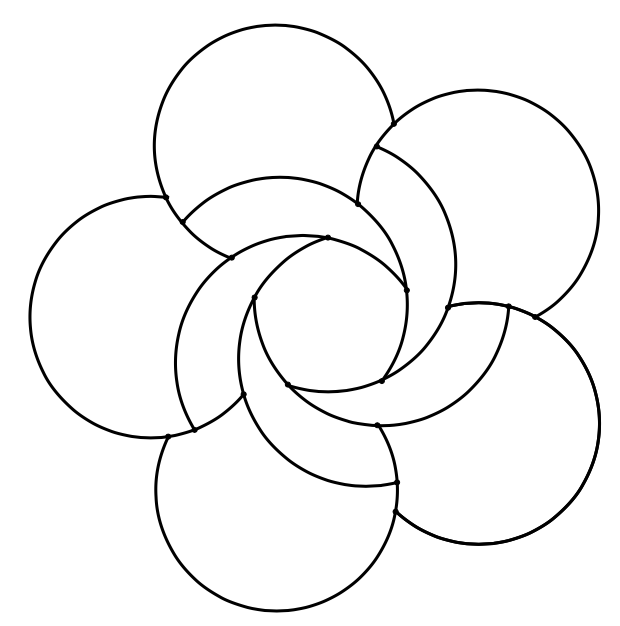
\includegraphics[height=3.5cm,natwidth=620,natheight=626]{Resources/Schulz.png}
\end{frame}

\begin{frame}
  \frametitle{\insertsubsection}
  \begin{itemize}
    \item Given a set ${\Pi = \lbrace P_1, \ldots, P_k \rbrace}$ of edge-disjoint paths \begin{itemize}
      \item ${V(\Pi) \coloneqq V(P_1) \cup \ldots \cup V(P_k)}$
      \item ${E(\Pi) \coloneqq E(P_1) \cupplus \ldots \cupplus E(P_k)}$
    \end{itemize}
    \item Drawing of ${\Pi}$ with circular arcs \begin{itemize}
      \item Drawing of ${G \coloneqq (V(\Pi), E(\Pi))}$ with circular arcs
      \item Each path ${P \in \Pi}$ is drawn as a circular arc ${\Gamma_P}$
    \end{itemize}
  \end{itemize}
  \centering
  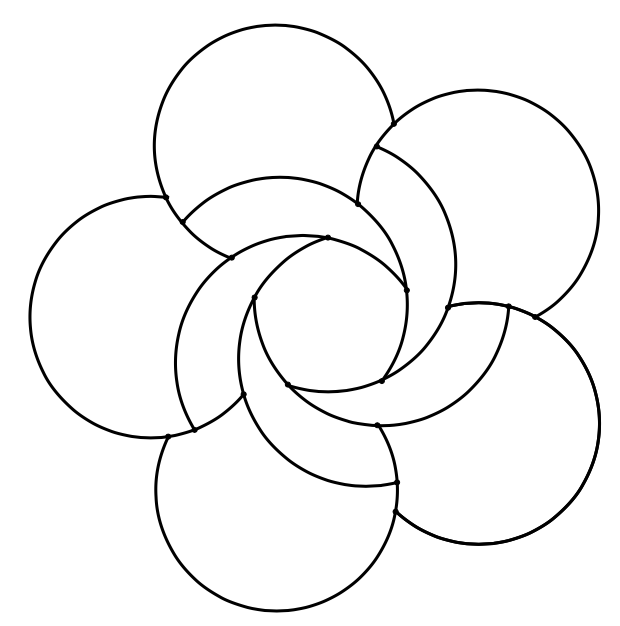
\includegraphics[height=3.5cm,natwidth=620,natheight=626]{Resources/Schulz.png}
\end{frame}

\subsection{Existence of Drawings}
\label{subsect:application-existence-of-drawings}

\begin{frame}
  \frametitle{\insertsubsection}
  \begin{itemize}
    \item Circles are determined by three distinct points
    \item Necessary condition: ${\abs{V(P_i) \cap V(P_j)} \leq 2 \quad \forall i \neq j}$ \begin{itemize}
      \item Condition is not sufficient!
    \end{itemize}
  \end{itemize}
  \begin{figure}
    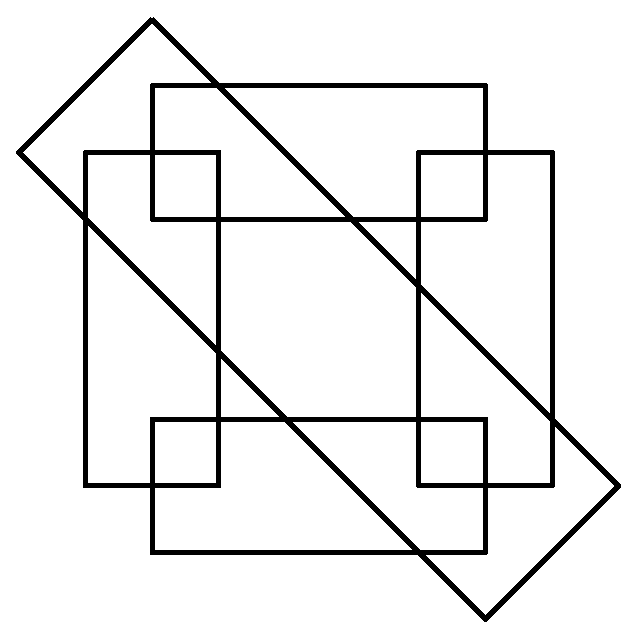
\includegraphics[height=3cm]{Resources/Arrangement-of-Pseudocircles}
    \quad
    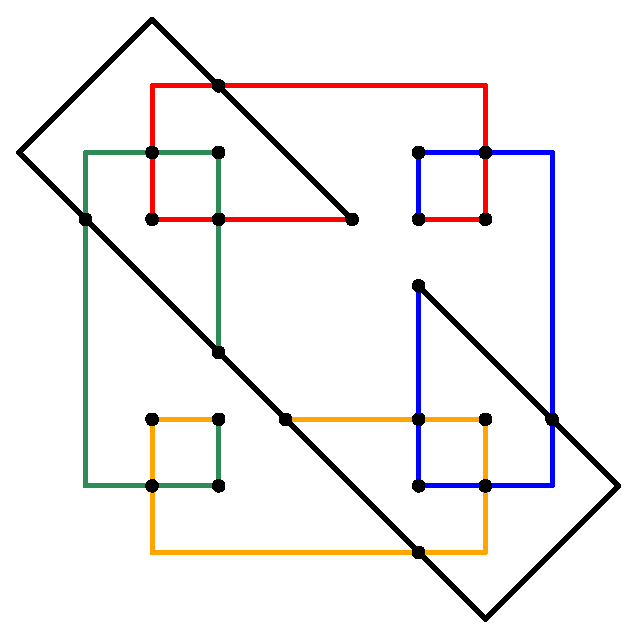
\includegraphics[height=3cm]{Resources/Arrangement-of-Pseudoarcs}
    \caption{An arrangement of pseudocircles that is not circleable (left) and a derived arrangement of pseudo circular arcs (right).}
  \end{figure}
\end{frame}

\begin{frame}
  \frametitle{\insertsubsection}
  \begin{itemize}
    \item Greedily realizable sequence of paths ${\Pi}$ \begin{itemize}
      \item Ordered sequence of edge-disjoint paths ${\Pi = (P_1, \ldots, P_k)}$
      \item ${V_\text{int}(P_i) \cap V(P_1 \cup \ldots \cup P_{i-1}) \stackrel{}{=} \varnothing, \quad i = 2 \ldots k}$
      \item Permits drawing with circular arcs using greedy algorithm
    \end{itemize}
  \end{itemize}
\end{frame}

\begin{frame}
  \frametitle{\insertsubsection}
  \begin{itemize}
    \item Greedily realizable sequence of paths ${\Pi}$ \begin{itemize}
      \item Ordered sequence of edge-disjoint paths ${\Pi = (P_1, \ldots, P_k)}$
      \item ${V_\text{int}(P_i) \cap V(P_1 \cup \ldots \cup P_{i-1}) \stackrel{}{=} \varnothing, \quad i = 2 \ldots k}$
      \item Permits drawing with circular arcs using greedy algorithm
    \end{itemize}
  \end{itemize}
  \begin{figure}
    \includegraphics<1>[height=4cm]{Resources/GreedyRealization-01}
    \includegraphics<2>[height=4cm]{Resources/GreedyRealization-02}
    \includegraphics<3>[height=4cm]{Resources/GreedyRealization-03}
    \includegraphics<4>[height=4cm]{Resources/GreedyRealization-04}
    \includegraphics<5>[height=4cm]{Resources/GreedyRealization-05}
    \includegraphics<6>[height=4cm]{Resources/GreedyRealization-06}
    \includegraphics<7>[height=4cm]{Resources/GreedyRealization-07}
    \includegraphics<8>[height=4cm]{Resources/GreedyRealization-08}
    \includegraphics<9>[height=4cm]{Resources/GreedyRealization-09}
    \includegraphics<10>[height=4cm]{Resources/GreedyRealization-10}
    \includegraphics<11>[height=4cm]{Resources/GreedyRealization-11}
    \caption{Greedy drawing of ${\Pi = ( \textit{abcde}, \textit{bfghd}, \textit{gijkl}, \textit{jmc} )}$}
  \end{figure}
\end{frame}

\begin{frame}
  \frametitle{\insertsubsection}
  \begin{itemize}
    \item Greedily realizable sequence of paths ${\Pi}$ \begin{itemize}
      \item Ordered sequence of edge-disjoint paths ${\Pi = (P_1, \ldots, P_k)}$
      \item ${V_\text{int}(P_i) \cap V(P_1 \cup \ldots \cup P_{i-1}) \stackrel{}{=} \varnothing, \quad i = 2 \ldots k}$
      \item Permits drawing with circular arcs using greedy algorithm
    \end{itemize}
    \item Characterization of vertices with respect to ${\Pi}$ \begin{itemize}
      \item Constrained vertices ${V_\text{c}(\Pi)}$: first appear as a path's internal vertex
      \item Unconstrained vertices ${V_\text{u}(\Pi)}$: first appear as a path's endpoint
    \end{itemize}
  \end{itemize}
\end{frame}

\subsection{Graph Decomposition}
\label{subsect:application-graph-decomposition}

\begin{frame}
  \frametitle{\insertsubsection}
  \begin{itemize}
    \item Find decomposition into greedily realizable sequence of (simple) paths
    \item Trivial decomposition ${\Pi = E}$ valid
    \item Non-trivial (greedy) graph decomposition \begin{itemize}
      \item Idea: append edges to working path until current head has been used before
    \end{itemize}
  \end{itemize}
  \centering
  \includegraphics<1>[height=4cm]{Resources/Graph-Decomposition-00.eps}
  \includegraphics<2>[height=4cm]{Resources/Graph-Decomposition-01.eps}
  \includegraphics<3>[height=4cm]{Resources/Graph-Decomposition-02.eps}
  \includegraphics<4>[height=4cm]{Resources/Graph-Decomposition-03.eps}
  \includegraphics<5>[height=4cm]{Resources/Graph-Decomposition-04.eps}
  \includegraphics<6>[height=4cm]{Resources/Graph-Decomposition-05.eps}
  \includegraphics<7>[height=4cm]{Resources/Graph-Decomposition-06.eps}
  \includegraphics<8>[height=4cm]{Resources/Graph-Decomposition-07.eps}
  \includegraphics<9>[height=4cm]{Resources/Graph-Decomposition-08.eps}
  \includegraphics<10>[height=4cm]{Resources/Graph-Decomposition-09.eps}
  \includegraphics<11>[height=4cm]{Resources/Graph-Decomposition-10.eps}
  \includegraphics<12>[height=4cm]{Resources/Graph-Decomposition-11.eps}
\end{frame}

\subsection{Generalized Coordinates}
\label{subsect:application-generalized-coordinates}

\begin{frame}
  \frametitle{\insertsubsection}
  \begin{itemize}
    \item Generalized coordinates \begin{itemize}
      \item \makebox[.5cm]{\hfill$x \colon$}\makebox[.9cm]{\hfill$V_\text{u}(\Pi)$} ${\to \mathbb{R}}$
      \item \makebox[.5cm]{\hfill$y \colon$}\makebox[.9cm]{\hfill$V_\text{u}(\Pi)$} ${\to \mathbb{R}}$
      \item \makebox[.5cm]{\hfill$\varphi \colon$}\makebox[.9cm]{\hfill$\Pi\phantom{)}$} ${\to (-180 \degrees, 180 \degrees)}$
      \item \makebox[.5cm]{\hfill$p \colon$}\makebox[.9cm]{\hfill$V_\text{c}(\Pi)$} ${\to (0, 1)}$
    \end{itemize}
  \end{itemize}
  \begin{figure}
    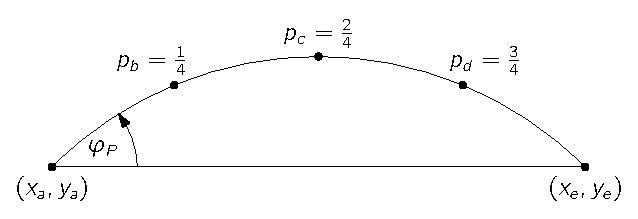
\includegraphics[height=2.0cm]{Resources/Generalized-Coordinates-Example.eps}
    \caption{Generalized coordinates for a single path ${P = abcde}$ with equi-length edges.}
  \end{figure}
\end{frame}

\begin{frame}[c]
  \frametitle{\insertsubsection}
  \begin{algorithm}[H]
    \caption{Transformation to Cartesian coordinates ${\vec{r}(v)}$}
    \SetKwData{CircularArc}{CircularArc}
    \SetKwData{PointForProgress}{pointForProgress}
    \ForEach{${v \in V_\text{u}(\Pi)}$}{
      ${\vec{r}(v) \gets (x({v}), y({v}))}$\;
    }
    \;
    \ForEach{${P = (v_1, \ldots, v_n) \in \Pi}$}{
      ${\Gamma(P) \gets \CircularArc(\vec{r}(v_1), \vec{r}(v_n), \varphi(P))}$\;
      \;
      \ForEach{${v \in (v_2, \ldots, v_{n-1})}$}{
        ${\vec{r}(v) \gets \Gamma(P).\PointForProgress(p(v))}$\;
      }
    }
    \;
  \end{algorithm}
\end{frame}

\subsection{Potential Energy}
\label{subsect:application-potential-energy}

\begin{frame}
  \frametitle{\insertsubsection}
  \begin{itemize}
    \item Vertex-Vertex repulsion \begin{itemize}
      \item Repulsive force based on Coulomb's law
      \item ${F_\text{rep}(d) \coloneqq c_1 \cdot \frac{1}{d^2}}$
    \end{itemize}
  \end{itemize}
  \begin{equation*}
    U_\text{rep}(u, v) \coloneqq{} \int\limits_{\infty}^{\mathclap{d(u, v)}} -F_\text{rep}(s) \differential{s}
  \end{equation*}
  \begin{itemize}
    \item Vertex-Vertex attraction \begin{itemize}
      \item Attractive force based on logarithmic spring
      \item ${F_\text{att}(l) \coloneqq -c_2 \cdot k \cdot \eval{\ln}{\frac{l}{k}}}$
    \end{itemize}
  \end{itemize}
  \begin{equation*}
    U_\text{att}(e) \coloneqq{} \int\limits_{k}^{\mathclap{l(\Gamma_e)}} -F_\text{att}(s) \differential{s}
  \end{equation*}
\end{frame}

\begin{frame}
  \frametitle{\insertsubsection}
  \begin{itemize}
    \item Order of vertices on a path \begin{itemize}
      \item Prevents intra-path overlapping edges
    \end{itemize}
  \end{itemize}
  \begin{equation*}
    U_\text{ord}(P) \coloneqq \begin{cases}
      0 & \text{if edges ${e \in E(P)}$ do not overlap} \\
      \infty & \text{otherwise}
    \end{cases} \hspace{0.25cm}
  \end{equation*}
  \begin{itemize}
    \item Vertex-Path repulsion \begin{itemize}
      \item Prevents unwanted vertex-edge intersections
      \item Prevents inter-path overlapping edges
    \end{itemize}
  \end{itemize}
  \begin{equation*}
    U_\text{int}(v, P) \coloneqq \begin{cases}
      c_3 \cdot \frac{1}{d(v, \Gamma_P)} & \text{if}~d(v, \Gamma_P) \neq 0 \\
      \infty & \text{otherwise}
    \end{cases}
  \end{equation*}
\end{frame}


\begin{frame}
  \frametitle{\insertsubsection}
  \begin{equation*}
  U \coloneqq
  \sum_{\mathclap{\substack{\lbrace u, v \rbrace \in V^2}}} U_\text{rep}(u, v)
  +
  \sum_{\mathclap{\substack{e \in E}}} U_\text{att}(e)
  +
  \sum_{\mathclap{\substack{P \in \Pi}}} U_\text{ord}(P)
  +
  \sum_{\mathclap{\substack{v \in V, P \in \Pi \\ v \notin V(P)}}} U_\text{int}(v, P)
  \end{equation*}
  \begin{itemize}
    \item Can be evaluated in ${\bigOh{\abs{V}^2 + \abs{E} + \abs{V} \cdot \abs{\Pi}}}$
    \item Optimization using hill climbing
  \end{itemize}
\end{frame}

\subsection{Results}
\label{subsect:application-results}

\newcommand{\drawing}[3]{\setlength\fboxsep{0pt}\colorbox{gray!10}{\makebox(75,75){\includegraphics[width=75pt,height=75pt,natwidth=#2,natheight=#3,keepaspectratio]{#1}}}}

\begin{frame}
  \frametitle{\insertsubsection}
  \begin{figure}
    \centerline{
      \drawing{Resources/Graph-10-09-1.pdf}{369}{291}\hspace{4pt}%
      \drawing{Resources/Graph-10-15-1.pdf}{267}{320}\hspace{4pt}%
      \drawing{Resources/Graph-10-20-1.pdf}{191}{145}\hspace{4pt}%
      \drawing{Resources/Graph-10-25-1.pdf}{122}{151}%
    }
    \vspace{3pt}
    \centerline{
      \drawing{Resources/Graph-10-09-2.pdf}{443}{196}\hspace{4pt}%
      \drawing{Resources/Graph-10-15-2.pdf}{253}{287}\hspace{4pt}%
      \drawing{Resources/Graph-10-20-2.pdf}{203}{165}\hspace{4pt}%
      \drawing{Resources/Graph-10-25-2.pdf}{203}{129}%
    }
    \caption{Drawings of graphs with 10 vertices and 9/15/20/25 edges; each with (bottom) and without (top) user adjustments.}
  \end{figure}
\end{frame}

\begin{frame}
  \frametitle{\insertsubsection}
  \begin{figure}
    \centerline{
      \drawing{Resources/Graph-15-14-1.pdf}{356}{362}\hspace{4pt}%
      \drawing{Resources/Graph-15-20-1.pdf}{356}{278}\hspace{4pt}%
      \drawing{Resources/Graph-15-25-1.pdf}{311}{248}\hspace{4pt}%
      \drawing{Resources/Graph-15-35-1.pdf}{276}{232}%
    }
    \vspace{3pt}
    \centerline{
      \drawing{Resources/Graph-15-14-2.pdf}{564}{404}\hspace{4pt}%
      \drawing{Resources/Graph-15-20-2.pdf}{341}{362}\hspace{4pt}%
      \drawing{Resources/Graph-15-25-2.pdf}{306}{271}\hspace{4pt}%
      \drawing{Resources/Graph-15-35-2.pdf}{262}{288}%
    }
    \caption{Drawings of graphs with 15 vertices and 14/20/25/35 edges; each with (bottom) and without (top) user adjustments.}
  \end{figure}
\end{frame}

\subsection{Demo}
\label{subsect:application-demo}

\begin{frame}
  \frametitle{\insertsubsection}
  \begin{itemize}
    \item Implemented as a Mac OS Application
    \item Written in Swift 3.0
  \end{itemize}
\end{frame}


\end{document}
